\documentclass[12pt]{article}
\usepackage[margin=1.2in]{geometry}
\usepackage[all]{nowidow}
\usepackage[hyperfigures=true, hidelinks, pdfhighlight=/N]{hyperref}
\usepackage[separate-uncertainty=true,group-digits=false]{siunitx}
\usepackage{graphicx,amsmath,physics,tabto,float,amssymb,pgfplots,verbatim,tcolorbox}
\usepackage{listings,xcolor,subfig,keyval2e,caption,import}
\numberwithin{equation}{section}
\definecolor{stringcolor}{HTML}{C792EA}
\definecolor{codeblue}{HTML}{2162DB}
\definecolor{commentcolor}{HTML}{4A6E46}
\lstdefinestyle{appendix}{
    basicstyle=\ttfamily\footnotesize,commentstyle=\color{commentcolor},keywordstyle=\color{codeblue},
    stringstyle=\color{stringcolor},showstringspaces=false,numbers=left,upquote=true,captionpos=t,
    abovecaptionskip=12pt,belowcaptionskip=12pt,language=Python,breaklines=true,frame=single}
\lstdefinestyle{inline}{
    basicstyle=\ttfamily\footnotesize,commentstyle=\color{commentcolor},keywordstyle=\color{codeblue},
    stringstyle=\color{stringcolor},showstringspaces=false,numbers=left,upquote=true,frame=tb,
    captionpos=b,language=Python}
\renewcommand{\lstlistingname}{Appendix}
\pgfplotsset{compat=1.17}

\title{Class Test 1}
\author{KDSMIL001 \; MAM2046W 2BP}
\date{\textbf{7 October 2020}}

\begin{document}
    \maketitle
    \begin{enumerate}
        \item \textbf{Heat Distribution}\newline
        Given the following:
        \begin{align*}
            \nabla^2 T&=\frac{1}{r}\frac{\partial }{\partial r}\left(r\frac{\partial T}{\partial r}\right)+\frac{1}{r^2}\frac{\partial^2 T}{\partial \theta^2}=0,\;0<r<30,\;0<\theta<\frac{\pi}{2}\\
            T(30,\theta)&=50,\;0<\theta<\frac{\pi}{2}\\
            |T(0,\theta)|&<\infty,\;0<\theta<\frac{\pi}{2}\\
            T(r,0)&=0,\;0<r<30\\
            T(r,\frac{\pi}{2})&=0,\;0<r<30
        \end{align*}
        \begin{enumerate}
            \item We separate $T(r,\theta)$ into two functions of only $r$ and $\theta$:
            \begin{equation*}
                T(r,\theta)=R(r)\Theta(\theta)
            \end{equation*}
            Our ICs and BCs become
            \begin{align*}
                R(30)&=50\\
                |R(0)|&<\infty\\
                \Theta(0)&=0\\
                \Theta(\frac{\pi}{2})&=0
            \end{align*}
            and our initial PDE then becomes
            \begin{align*}
                0&=\frac{1}{r}\frac{\partial }{\partial r}\left(r\frac{\partial R\Theta}{\partial r}\right)+\frac{1}{r^2}\frac{\partial^2 R\Theta}{\partial \theta^2}\\
                \implies \frac{\Theta}{r}\frac{d}{d r}\left(r\frac{d R}{d r}\right)&=-\frac{R}{r^2}\frac{d^2 \Theta}{d \theta^2}\\
                \implies \frac{1}{R}\left[r^2\frac{d^2R}{dr^2}+r\frac{dR}{dr}\right]&=-\frac{1}{\Theta}\frac{d^2 \Theta}{d\theta^2}
            \end{align*}
            We then set each ODE to the same constant $\lambda$, since they are equal, giving us 
            \begin{align*}
                \frac{d^2\Theta}{d\theta^2}&=-\lambda \Theta\\
                r^2\frac{d^2R}{dr^2}+r\frac{dR}{dr}-\lambda R&=0
            \end{align*}
            Starting with $\Theta$, we know the solutions to this type of equation. For $\lambda>0$ we have
            \begin{equation*}
                \Theta(\theta)=A\sin(\sqrt\lambda \theta)+B\cos(\sqrt\lambda \theta)
            \end{equation*}
            Applying the BCs we get
            \begin{align*}
                \Theta(0)&=A*0+B*1=0\\
                \implies B&=0\\
                \Theta(\frac{\pi}{2})&=A\sin(\sqrt\lambda\frac{\pi}{2})=0\\
                \implies \sqrt\lambda\frac{\pi}{2}&=n\pi,\; n\in\mathbb{N}\\
                \implies \lambda&=4\pi^2,\; n\in\mathbb{N}
            \end{align*}
            And so we have a solution to the $\Theta$ ODE for $\lambda>0$:
            \begin{equation*}
                \Theta(\theta)=A\sin(2n\theta),\; n\in\mathbb{N}
            \end{equation*}
            We know that this equation has no solution for $\lambda<0$, and the solution for $\lambda=0$ is $\Theta=C,\; C\in\mathbb{R}$.\newline
            Moving on to the $R$ ODE, we have
            \begin{equation*}
                r^2\frac{d^2R}{dr^2}+r\frac{dR}{dr}-\lambda R=0
            \end{equation*}
            which is an Euler ODE, the standard ansatz for which is $R=r^s,\; r>0$, so it's always valid in our case. Using this ansatz we find 
            \begin{align*}
                r^2[s(s-1)r^{s-2}]+r[sr^{s-1}]-4n^2r^s&=0\\
                \implies s^2-4n^2&=0\\
                \implies s&=\pm 2n
            \end{align*}
            For an Euler ODE the solutions usually depend on $n$, but in our case $n>0$ so we only examine that case. For $n\neq0$, Euler ODEs have the solution:
            \begin{equation*}
                R(r)=Dr^{2n}+Er^{-2n}
            \end{equation*}
            Here is where our boundedness condition comes in. If we examine the solution as $r\rightarrow 0$, we can see that it explodes 
            to $\infty$, but since we know that $|R(0)|<\infty$, we must have that $E=0$ to stop this blowing up. So for $n\neq0$
            \begin{equation*}
                R(r)=Dr^{2n}
            \end{equation*}
            Recall we had $T=R\Theta$, so our solution is
            \begin{align*}
                T_n(r,\theta)&=A\sin(2n\theta)Dr^{2n}\\
                &=C\sin(2n\theta)r^{2n}
            \end{align*}
            And we have the infinite series representation:
            \begin{equation*}
                T(r,\theta)=\sum_{n=1}^\infty C_n \sin(2n\theta)r^{2n}
            \end{equation*}

            \item Applying the final BC, we have
            \begin{align*}
                T(30,\theta)=50&=\sum_{n=1}^\infty C_n \sin(2n\theta)30^{2n}\\
                \implies 50 \sin(2m\theta)&=\sum_{n=1}^\infty C_n 30^{2n}\sin(2n\theta)\sin(2m\theta)\\
                \implies \int_0^{\frac{\pi}{2}}50 \sin(2m\theta) d\theta&= \sum_{n=1}^\infty C_n 30^{2n}\int_0^{\frac{\pi}{2}}\sin(2n\theta)\sin(2m\theta)d\theta
            \end{align*}
            By orthogonality relations, the $\int_0^{\frac{\pi}{2}}\sin(2n\theta)\sin(2m\theta)d\theta$ term goes to 0 for all $n\neq m$, which simplifies it down to
            \begin{align*}
                \int_0^{\frac{\pi}{2}}50 \sin(2m\theta) d\theta&=C_m 30^{2m}\int_0^{\frac{\pi}{2}}\sin^2(2m\theta)d\theta\\
                &=C_m 30^{2m} \frac{\pi}{4}\\
                \implies C_m&= \frac{4}{30^{2m}\pi} \int_0^{\frac{\pi}{2}}50 \sin(2m\theta) d\theta
            \end{align*}
        \end{enumerate}
        
        \item \textbf{Fourier Series}\newline
        Given the function:
        \begin{equation*}
            f(x)=
            \begin{cases}
                0 & -\pi\leq x<0\\
                x^2 & 0\leq x\leq\pi
            \end{cases}
        \end{equation*}
        \begin{enumerate}
            \item The Fourier Series of $f(x)$ will look like the following
            \begin{figure}[H]
                \begin{center}
                   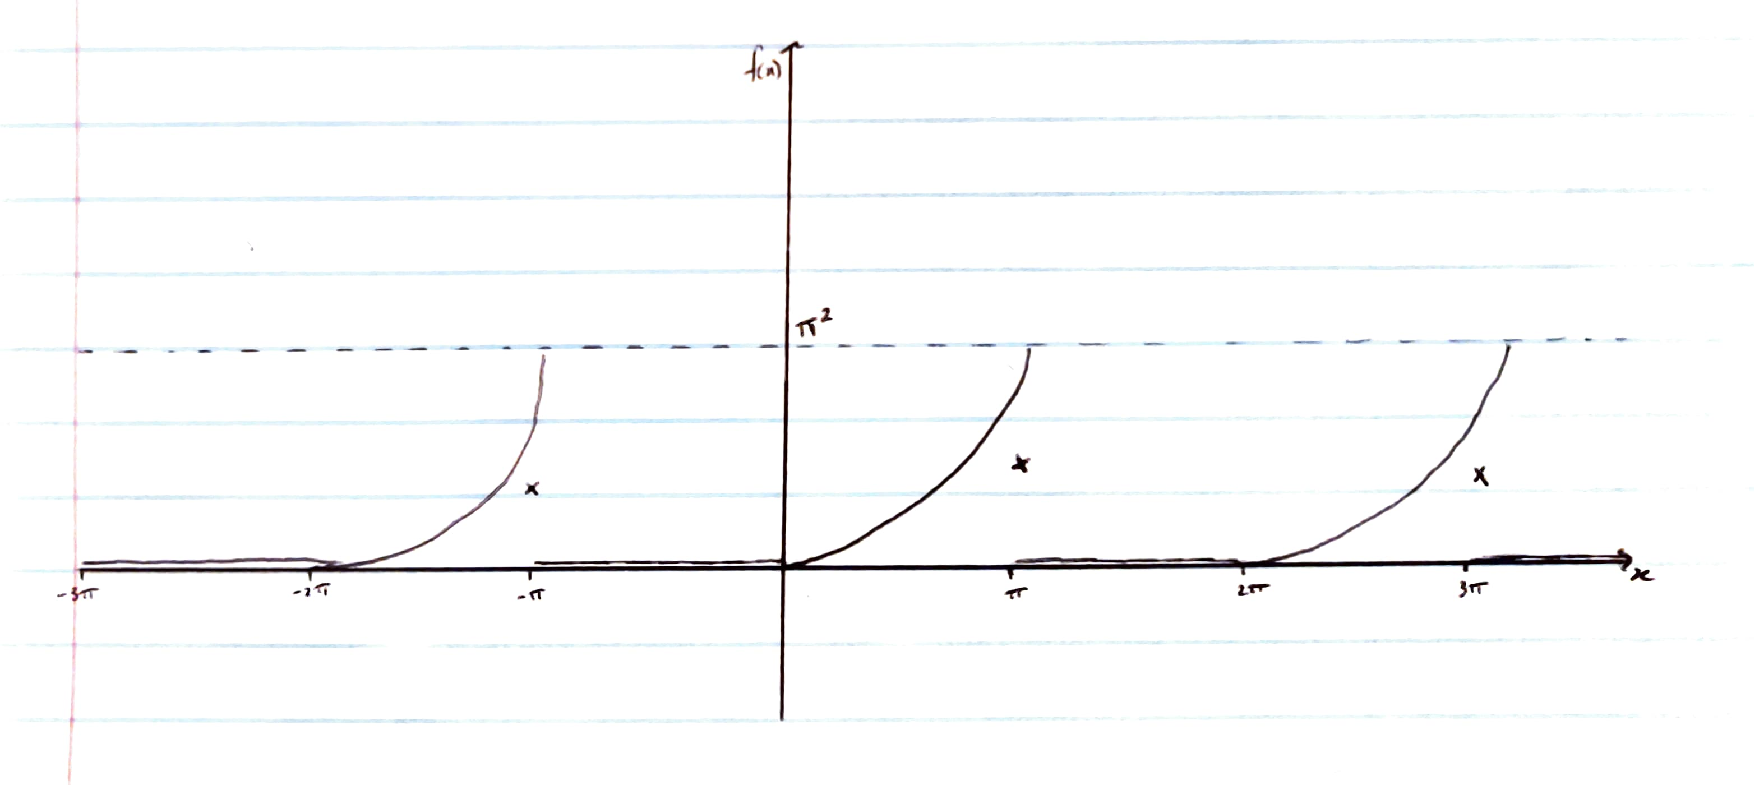
\includegraphics[width=1\textwidth]{CT1Plot.pdf}
                   \caption{Fourier Series plot of $f(x)$}
                   \label{fig:FourierPlot}
                \end{center}
            \end{figure}
            
            \item The Fourier Coefficients are given by 
            \begin{align*}
                A_0&=\frac{1}{2L}\int_{-L}^Lf(x)dx\\
                A_m&=\frac{1}{L}\int_{-L}^L f(x)\cos(\frac{m\pi x}{L})dx\\
                B_m&=\frac{1}{L}\int_{-L}^L f(x)\sin(\frac{m\pi x}{L})dx
            \end{align*}
            Starting with $A_0$:
            \begin{align*}
                A_0&=\frac{1}{4\pi}\left[\int_{-\pi}^0 0dx+\int_0^\pi x^2 dx\right]\\
                &=\frac{1}{4\pi}\left[\frac{x^3}{3}\right]_0^\pi\\
                &=\frac{1}{4\pi}\frac{\pi^3}{3}\\
                A_0&=\frac{\pi^2}{12}
            \end{align*}
            Now 
            \begin{align*}
                A_m&=\frac{1}{2\pi}\left[\int_{-\pi}^0 0 dx +\int_{0}^\pi x^2\cos(\frac{m x}{2})dx\right]\\
                &=\frac{1}{2\pi} \int_{0}^\pi x^2\cos(\frac{m x}{2})dx\\
                &=\frac{(\pi^2m^2-8)\sin(\frac{\pi m}{2})+4\pi m\cos(\frac{\pi m}{2})}{m^3 \pi}
            \end{align*}
            And
            \begin{align*}
                B_m&=\frac{1}{2\pi}\left[\int_{-\pi}^0 0 dx +\int_{0}^\pi x^2\sin(\frac{m x}{2})dx\right]\\
                &=\frac{1}{2\pi} \int_{0}^\pi x^2\sin(\frac{m x}{2})dx\\
                &=-\frac{((\pi^2m^2-8)\cos(\frac{\pi m}{2})-4\pi m\sin(\frac{\pi m}{2})+8)}{m^3 \pi}
            \end{align*}
            Since the original function is piecewise-smooth but has jump discontinuities, we know that the Fourier Series will converge to $f(x)$ within the bounds 
            of the domain, and will converge to $\frac{pi^2}{2}$ at the discontinuities. 

            \item The Fourier Series can not be differentiated term by term as 
            \begin{equation*}
                f(-\pi)=0\neq f(\pi)=\pi^2
            \end{equation*}
        \end{enumerate}
    \end{enumerate}

\end{document}